% 矩阵一节：矩阵的表示与常见矩阵；加法与数乘、转置、矩阵与向量的乘积、矩阵乘法、逐项乘积（各自先定义、再整理性质）；初等行变换；逆矩阵；矩阵的幂。行列式、迹与Frobenius内积见下一节。

\section{矩阵}
\label{sec:ls-matrices}

一批样本的特征排成一张数表以后，常要对每个样本用同一组权重求加权和。矩阵就是这样的数表，矩阵乘法则一次写出这些加权和。

本节先规定矩阵的写法，再逐个讨论矩阵的运算，每种运算都先给定义、再整理性质。重点是矩阵乘法：它保留了实数乘法的结合律与分配律，却失去了交换律与消去律。最后三小节用乘法回答三个具体问题：怎样用可撤销的步骤化简矩阵，怎样撤销一次乘法，怎样记录同一矩阵的反复作用。

\subsection{矩阵的表示与常见矩阵}
\label{sec:ls-matrix-representation}

向量中的一个数用一个索引定位。数表中的一个数要由所在的行与列共同确定，需要两个索引。

\paragraph{矩阵、元素与形状}
$m$行$d$列的实数表称为矩阵（matrix），记为$\bm A\in\mathbb R^{m\times d}$。第$i$行、第$j$列的元素记为$\bm A_{i,j}$，不致混淆时也写作$a_{i,j}$。$m\times d$称为矩阵的形状，行数写在前，列数写在后。$\bm A_{i,:}$表示第$i$行，$\bm A_{:,j}$表示第$j$列，冒号表示取该方向上的全部位置；第$j$列是$m$维列向量，第$i$行是$d$维行向量。例如在
\[
 \bm A=\begin{bmatrix}1&2&3\\4&5&6\end{bmatrix}\in\mathbb R^{2\times3}
\]
中，$\bm A_{2,1}=4$，第一行$\bm A_{1,:}=\left[\begin{smallmatrix}1&2&3\end{smallmatrix}\right]$，第三列$\bm A_{:,3}=(3,6)^\top$。

两个矩阵相等，是指形状相同且每个对应元素相等。

只有一行的矩阵就是行向量，只有一列的矩阵就是列向量，所以向量可以看作矩阵的特例。

\paragraph{设计矩阵}
用矩阵记录数据时，通常让每行对应一个样本，每列对应一个特征，这样的矩阵称为设计矩阵。把示例~\ref{ex:ls-nearly-collinear-features}中的$\bm c_1,\bm c_2$并排作为两列，得到三个样本、两个特征的设计矩阵
\begin{equation}
\bm X_{\varepsilon}
 =\begin{bmatrix}\bm c_1&\bm c_2\end{bmatrix}
 =\begin{bmatrix}1&1\\1&1+\varepsilon\\1&1-\varepsilon\end{bmatrix},\qquad
 \bm c_2=\bm c_1+\varepsilon\bm q.
\label{eq:linear-algebra-nearly-collinear-design}
\end{equation}
后面各章反复用这个矩阵考察两列几乎相同时会出现什么问题。

\subsubsection{常见矩阵}
\label{sec:prelim-common-matrices}

有些矩阵的元素有固定的分布模式：大部分位置为零，或者关于主对角线对称。这些模式会让后面的运算大为简化。下面按元素的位置与取值逐类给出定义和例子；它们在矩阵乘法下呈现的固定模式，在第~\ref{sec:ls-common-matrix-products}节随乘法讨论。依赖内积的正交矩阵与正定矩阵在第~\ref{chap:normed-inner-product-spaces}章建立。

\paragraph{方阵}
行数等于列数的矩阵称为方阵（square matrix），$n\times n$方阵也称$n$阶方阵。位置$(i,i)$上的元素组成主对角线。例如
\[
 \begin{bmatrix}1&2\\3&4\end{bmatrix}
\]
是二阶方阵，主对角元素为$1$和$4$；$2\times3$矩阵不是方阵。下面的对角矩阵和三角矩阵都限定为方阵。

\paragraph{零矩阵}
全部元素都为$0$的矩阵称为零矩阵（zero matrix），记作$\bm0$。它不要求是方阵，需要时写明形状，例如
\[
 \bm0_{2\times3}=\begin{bmatrix}0&0&0\\0&0&0\end{bmatrix}.
\]

\paragraph{对角矩阵}
主对角线以外的元素都为$0$的方阵称为对角矩阵（diagonal matrix），记为$\operatorname{diag}(d_1,\ldots,d_n)$。主对角元素本身可以为$0$。例如
\[
\begin{gathered}
\operatorname{diag}(2,0)=\begin{bmatrix}2&0\\0&0\end{bmatrix},\\
\operatorname{diag}(1,-1,3)=\begin{bmatrix}1&0&0\\0&-1&0\\0&0&3\end{bmatrix}.
\end{gathered}
\]

\paragraph{单位矩阵}
主对角元素全为$1$的对角矩阵称为单位矩阵（identity matrix），记为$\bm I_n$；不必强调阶数时写作$\bm I$。它的第$j$列就是标准坐标向量$\bm e_j$。例如
\[
 \bm I_3=\begin{bmatrix}1&0&0\\0&1&0\\0&0&1\end{bmatrix}=\begin{bmatrix}\bm e_1&\bm e_2&\bm e_3\end{bmatrix}.
\]

\paragraph{上三角矩阵}
$i>j$时$\bm A_{i,j}=0$的方阵称为上三角矩阵（upper triangular matrix）。它的主对角线以下全为零，非零元素只可能出现在主对角线及其上方。例如
\[
 \begin{bmatrix}1&2&3\\0&4&5\\0&0&6\end{bmatrix}.
\]

\paragraph{下三角矩阵}
$i<j$时$\bm A_{i,j}=0$的方阵称为下三角矩阵（lower triangular matrix），它的主对角线以上全为零。例如
\[
 \begin{bmatrix}1&0&0\\2&3&0\\4&5&6\end{bmatrix}.
\]
对角矩阵既是上三角矩阵，也是下三角矩阵。

\paragraph{对称矩阵}
若方阵满足$\bm A_{i,j}=\bm A_{j,i}$对全部$i,j$成立，就称为对称矩阵（symmetric matrix）。它的元素关于主对角线镜像对称。定义转置以后，这个条件可以写作$\bm A^\top=\bm A$。例如
\[
\begin{bmatrix}1&2\\2&3\end{bmatrix},\qquad
\begin{bmatrix}4&-1&0\\-1&2&5\\0&5&1\end{bmatrix}.
\]
对角矩阵都是对称矩阵。

\paragraph{置换矩阵}
把单位矩阵的各列重新排列，得到的方阵称为置换矩阵（permutation matrix）。它的每行、每列恰有一个$1$，其余元素为$0$。例如
\[
\begin{bmatrix}0&1\\1&0\end{bmatrix}=\begin{bmatrix}\bm e_2&\bm e_1\end{bmatrix},\qquad
\begin{bmatrix}0&0&1\\1&0&0\\0&1&0\end{bmatrix}=\begin{bmatrix}\bm e_2&\bm e_3&\bm e_1\end{bmatrix}.
\]
定义矩阵乘法以后会看到，第一个矩阵乘在平面向量上，交换它的两个坐标。

\subsection{加法与数乘}
\label{sec:ls-matrix-addition-scaling}

矩阵的加法与数乘沿用向量的逐项规则。同形矩阵$\bm A,\bm B\in\mathbb R^{m\times n}$逐项相加减，数乘把每个元素乘以同一个实数$c$：
\[
 \begin{gathered}
(\bm A\pm\bm B)_{i,j}=a_{i,j}\pm b_{i,j},\\
(c\bm A)_{i,j}=ca_{i,j}.
 \end{gathered}
\]
结果的形状不变。下面是一组二阶矩阵的算例。
\begin{example}[矩阵的加法、减法与数乘]
\label{ex:ls-matrix-addition-scaling}
取
\[
\bm A=\begin{pmatrix}1&2\\3&4\end{pmatrix},\qquad
\bm B=\begin{pmatrix}0&1\\-1&2\end{pmatrix},\qquad
c=3.
\]
每个位置上的元素单独运算：
\[
\begin{gathered}
\bm A+\bm B=\begin{pmatrix}1&3\\2&6\end{pmatrix},\\
\bm A-\bm B=\begin{pmatrix}1&1\\4&2\end{pmatrix},\\
3\bm A=\begin{pmatrix}3&6\\9&12\end{pmatrix}.
\end{gathered}
\]
以$(2,1)$位置为例，$\bm A+\bm B$在这里是$3+(-1)=2$，$\bm A-\bm B$在这里是$3-(-1)=4$，都只用到$\bm A$与$\bm B$的$(2,1)$元。三个结果仍是$2\times2$矩阵，这和向量的逐坐标运算完全一样。
\end{example}
与向量一样，两个矩阵相加，要求形状相同、对应位置含义相同。$2\times3$矩阵与$3\times2$矩阵的元素个数相同，却不能相加。同形矩阵的线性组合按同样方式定义。

\subsubsection{加法与数乘的性质}
同形矩阵逐项相加与数乘，所以向量的八条规则在每个位置上照样成立。对同形矩阵$\bm A,\bm B,\bm C$和实数$a,b$，
\[
\begin{aligned}
 &\bm A+\bm B=\bm B+\bm A, && (\bm A+\bm B)+\bm C=\bm A+(\bm B+\bm C),\\
 &\bm A+\bm0=\bm A, && \bm A+(-\bm A)=\bm0,\\
 &a(b\bm A)=(ab)\bm A, && 1\bm A=\bm A,\\
 &(a+b)\bm A=a\bm A+b\bm A, && a(\bm A+\bm B)=a\bm A+a\bm B.
\end{aligned}
\]
每一条都可以在任一位置$(i,j)$上用实数运算直接验证。

\subsection{转置}
\label{sec:ls-matrix-transpose}

转置交换行与列：$\bm A\in\mathbb R^{m\times n}$的元素$a_{i,j}$原样搬到$\bm A^\top\in\mathbb R^{n\times m}$的位置$(j,i)$，
\[
 (\bm A^\top)_{j,i}=\bm A_{i,j}.
\]
形状随之交换，数值不变，原来的第$i$行成为第$i$列。把列向量看作$d\times1$矩阵，这一定义与上一节向量的转置一致。下面的例子显示行怎样变成列。
\begin{example}[转置一个$2\times3$矩阵]
\label{ex:ls-transpose-two-by-three}
把
\[
 \bm A=\begin{bmatrix}1&2&3\\4&5&6\end{bmatrix}\in\mathbb R^{2\times3}
\]
的每个$(i,j)$元搬到$(j,i)$位置，得到
\[
 \bm A^\top=\begin{bmatrix}1&4\\2&5\\3&6\end{bmatrix}\in\mathbb R^{3\times2}.
\]
$\bm A$的第一行$(1,2,3)$竖了起来，成为$\bm A^\top$的第一列；第二行$(4,5,6)$成为第二列。形状也随之由$2\times3$变为$3\times2$。
\end{example}

\subsubsection{转置的性质}

转置只改变元素的位置。下面两条说明它与加法、数乘的关系，以及转置两次的结果；它与矩阵乘积的关系要等定义了矩阵乘法以后，在第~\ref{sec:ls-reshaping}节讨论。

\paragraph{与加法、数乘交换}
\[
 \begin{gathered}
(\bm A+\bm B)^\top=\bm A^\top+\bm B^\top,\\
(c\bm A)^\top=c\bm A^\top.
 \end{gathered}
\]
转置只搬动元素，逐项运算的结果搬到新位置后不变。

\paragraph{转置的转置}
\[
 (\bm A^\top)^\top=\bm A.
\]
转置两次，$(i,j)$元先搬到$(j,i)$，再搬回$(i,j)$，每个元素回到原位。

\subsection{矩阵与向量的乘积}
\label{sec:prelim-matrix-records-prediction}

设$n$次观测的输入排成设计矩阵$\bm X\in\mathbb R^{n\times d}$，权重排成$\bm w\in\mathbb R^d$。线性预测对第$i$次观测计算加权和$\sum_j x_{i,j}w_j$，也就是$\bm X$的第$i$行与$\bm w$的内积。矩阵与向量的乘积把这$n$个加权和一次写出。对$\bm A\in\mathbb R^{m\times d}$与$\bm u\in\mathbb R^d$，$\bm A\bm u$是$m$维列向量，
\begin{equation}
(\bm A\bm u)_i=\sum_{j=1}^d\bm A_{i,j}u_j,\qquad i=1,\ldots,m.
\label{eq:prelim-matrix-prediction}
\end{equation}
这里矩阵的列数必须等于向量的维数。

同一个乘积可以按行算，也可以按列算，两者结果相同：
\begin{itemize}
 \item 按行算：输出的第$i$个坐标是第$i$行与$\bm u$的内积。
 \item 按列算：式~\eqref{eq:prelim-matrix-prediction}中，$u_j$乘的恰好是第$j$列的各个元素，所以
 \[
  \bm A\bm u=u_1\bm A_{:,1}+u_2\bm A_{:,2}+\cdots+u_d\bm A_{:,d},
 \]
 即乘积是矩阵各列以$u_j$为系数的线性组合。
\end{itemize}
按列算还说明，$\bm e_j$只有第$j$个系数为$1$，所以$\bm A\bm e_j=\bm A_{:,j}$：乘第$j$个标准坐标向量，就取出第$j$列。对贯穿例，按列算得$\bm X_\varepsilon\bm w=w_1\bm c_1+w_2\bm c_2$，预测是两个特征取值向量的线性组合。

下面用一个二阶例子核对两种算法给出同一结果。
\begin{example}[按行与按列计算矩阵与向量的乘积]
\label{ex:ls-matrix-vector-rows-columns}
取
\[
\bm A=\begin{bmatrix}2&1\\0&3\end{bmatrix},\qquad
\bm u=\begin{bmatrix}1\\1\end{bmatrix}.
\]
下面第一行算式按行算，每个坐标是$\bm A$的一行与$\bm u$的内积；第二行算式按列算，把$\bm A$的两列以$u_1=u_2=1$为系数组合起来：
\[
\begin{gathered}
\bm A\bm u
 =\begin{bmatrix}2\cdot1+1\cdot1\\0\cdot1+3\cdot1\end{bmatrix}
 =\begin{bmatrix}3\\3\end{bmatrix},\\
\bm A\bm u=1\begin{bmatrix}2\\0\end{bmatrix}+1\begin{bmatrix}1\\3\end{bmatrix}
 =\begin{bmatrix}3\\3\end{bmatrix}.
\end{gathered}
\]
两种算法都得到$(3,3)^\top$。按行算的每一项乘积，在按列算中也恰好出现一次，只是加起来的顺序不同。
\end{example}

用于数据时，一次矩阵与向量的乘积给出全部样本的预测。下面以一次函数为例。
\begin{example}[用矩阵与向量的乘积计算一次函数的取值与残差]
\label{ex:ls-affine-predictions}
设要在$x=1,2,3$三处计算一次函数$ax+b$的值。把三处的$x$排成第一列、再补上一列$1$，系数排成向量，即
\[
\bm X=\begin{pmatrix}1&1\\2&1\\3&1\end{pmatrix},\qquad
\bm w=\begin{pmatrix}a\\b\end{pmatrix}.
\]
按行算，
\[
 \bm X\bm w=\begin{pmatrix}1\cdot a+1\cdot b\\2\cdot a+1\cdot b\\3\cdot a+1\cdot b\end{pmatrix}=\begin{pmatrix}a+b\\2a+b\\3a+b\end{pmatrix}.
\]
$\bm X\bm w$的三个坐标正是三处的函数值；第二列全为$1$，使每行都加上同一个截距$b$。再把三处的观测输出排成$\bm y=(y_1,y_2,y_3)^\top$，全部残差就是$\bm X\bm w-\bm y$，平方误差总和写成
\[
 \sum_{i=1}^3\bigl(a\,i+b-y_i\bigr)^2
 =\lVert\bm X\bm w-\bm y\rVert_2^2.
\]
左侧逐处求函数值、减去观测、平方后相加；右侧把同样的计算写成残差向量长度的平方。

这里只用到乘积按行展开和长度的定义，与样本数、特征数无关。$n$个样本、$d$个特征时同样有
\[
 \sum_{i=1}^n\Bigl(\sum_{j=1}^d x_{i,j}w_j-y_i\Bigr)^2=\lVert\bm X\bm w-\bm y\rVert_2^2.
\]
于是一次矩阵与向量的乘积给出全部预测，平方误差总和则是残差向量长度的平方。
\end{example}

\subsection{矩阵乘法}
\label{sec:ls-matrix-operations}
\label{sec:ls-multiplication}
\label{sec:prelim-linear-actions-composition}

两次加权求和可能接连进行。设$\bm B\in\mathbb R^{d\times k}$，$\bm A\in\mathbb R^{m\times d}$。对$\bm x\in\mathbb R^k$，先算$\bm y=\bm B\bm x$，再算$\bm z=\bm A\bm y$。这就是两个映射的复合：$\bm x\mapsto\bm B\bm x$的输出$\bm y$恰好落在$\bm y\mapsto\bm A\bm y$的定义域$\mathbb R^d$中，复合映射把$\bm x$直接送到$\bm A(\bm B\bm x)$；映射复合的一般定义可参考\BookChapterRef{chap:sets-relations-maps}{卷一“集合、关系与映射”一章}。

逐坐标代入，再交换有限求和的次序，得到
\begin{equation}
 z_i=\sum_{\ell=1}^d a_{i,\ell}\sum_{j=1}^k b_{\ell,j}x_j
 =\sum_{j=1}^k\left(\sum_{\ell=1}^d a_{i,\ell}b_{\ell,j}\right)x_j.
 \label{eq:linear-algebra-matrix-product}
\end{equation}
可见$\bm z$仍是$\bm x$各坐标的加权和。把括号中的系数排成一张表，就得到矩阵乘法的定义。

对$\bm A\in\mathbb R^{m\times d}$与$\bm B\in\mathbb R^{d\times k}$，乘积$\bm A\bm B\in\mathbb R^{m\times k}$定义为
\begin{equation}
 (\bm A\bm B)_{i,j}=\sum_{\ell=1}^d\bm A_{i,\ell}\bm B_{\ell,j}.
 \label{eq:prelim-matrix-composition}
\end{equation}
左矩阵的列数必须等于右矩阵的行数。第$(i,j)$项取左矩阵的第$i$行与右矩阵的第$j$列，逐项相乘后相加。被求和掉的公共维数$d$，就是中间结果$\bm y$的维数。
$\bm B$只有一列时，式~\eqref{eq:prelim-matrix-composition}就是式~\eqref{eq:prelim-matrix-prediction}。两个向量的内积$\bm x^\top\bm y$是$1\times d$矩阵与$d\times1$矩阵的乘积，结果是$1\times1$矩阵，我们把它与其唯一的元素等同看待。

非方阵相乘时，写出每个因子的形状尤其有用。以$2\times3$矩阵乘$3\times2$矩阵为例，
\[
 \begin{aligned}
 &\begin{pmatrix}1&2&0\\0&1&3\end{pmatrix}
 \begin{pmatrix}1&0\\2&1\\1&-1\end{pmatrix}\\
 &=\begin{pmatrix}1\cdot1+2\cdot2+0\cdot1&1\cdot0+2\cdot1+0\cdot(-1)\\
 0\cdot1+1\cdot2+3\cdot1&0\cdot0+1\cdot1+3\cdot(-1)\end{pmatrix}\\
 &=\begin{pmatrix}5&2\\5&-2\end{pmatrix}.
 \end{aligned}
\]
左矩阵的列数与右矩阵的行数都是$3$，乘法有定义；输出保留左矩阵的$2$行和右矩阵的$2$列。若这两个数不相等，行与列就无法逐项配对。

\subsubsection{矩阵乘法的性质}
\label{sec:ls-matrix-operation-properties}

矩阵乘法保留了实数乘法的结合律和分配律，但一般不满足交换律和消去律。下面逐条核对，并检查每条规则对形状的要求。

\paragraph{单位乘}
\[
\bm I_m\bm A=\bm A=\bm A\bm I_d,\qquad
\bm A\in\mathbb R^{m\times d}.
\]
$\bm I_m$的第$i$行是$\bm e_i^\top$，它乘$\bm A$的第$j$列，取出$a_{i,j}$；右乘同理。单位矩阵在矩阵乘法中的作用，相当于数$1$在实数乘法中的作用。

\paragraph{零乘}
\[
 \bm0\bm A=\bm0,\qquad\bm A\bm0=\bm0.
\]
乘积的每个元素都是若干乘积之和。一个因子全为零时，每一项都为零。各个零矩阵的形状由相乘的另一个因子决定。

反过来不成立：由$\bm A\bm B=\bm0$不能推出$\bm A=\bm0$或$\bm B=\bm0$。下面是一个反例。
\begin{example}[反例：两个非零矩阵的乘积为零]
\label{ex:ls-zero-product-nonzero-factors}
两个二阶矩阵
\[
\bm A=\begin{bmatrix}1&0\\0&0\end{bmatrix},\qquad
\bm B=\begin{bmatrix}0&0\\1&0\end{bmatrix}
\]
各有一个非零元，都不是零矩阵。按定义相乘，
\[
 \bm A\bm B=\begin{bmatrix}1\cdot0+0\cdot1&1\cdot0+0\cdot0\\0\cdot0+0\cdot1&0\cdot0+0\cdot0\end{bmatrix}=\begin{bmatrix}0&0\\0&0\end{bmatrix}.
\]
四个元素全为零。可见两个非零因子的乘积可以是零矩阵，实数中“乘积为零则必有一个因子为零”的推理不能搬到矩阵上。
\end{example}
按列看可以说明原因。由乘积的元素公式，$\bm A\bm B$的第$j$列就是$\bm A$乘$\bm B$的第$j$列。所以$\bm A\bm B=\bm0$恰好意味着$\bm B$的每一列$\bm b$都满足$\bm A\bm b=\bm0$。上例中$\bm A$只保留第一个坐标、把第二个坐标清零；$\bm B$的第一列$(0,1)^\top$只有第二个坐标非零，第二列为零，于是两列都被$\bm A$清零。

\paragraph{结合律}
\[
 (\bm A\bm B)\bm C=\bm A(\bm B\bm C).
\]
按式~\eqref{eq:prelim-matrix-composition}展开，两边的第$(i,j)$项都是$\sum_k\sum_l a_{i,k}b_{k,l}c_{l,j}$，只是两个有限求和的次序不同。从映射的角度看，这就是复合的结合律：先作用$\bm C$、再作用$\bm B$、最后作用$\bm A$，无论先把哪两步合并，得到的都是同一个映射。取$\bm C$为列向量$\bm x$，得$(\bm A\bm B)\bm x=\bm A(\bm B\bm x)$：用乘积作用一次，等于先用$\bm B$、再用$\bm A$作用。这正是式~\eqref{eq:linear-algebra-matrix-product}引出乘法定义时的计算。有了结合律，多个形状相容的矩阵连乘时不必加括号。

\paragraph{分配律与数乘相容}
\[
 \begin{gathered}
\bm A(\bm B+\bm C)=\bm A\bm B+\bm A\bm C,\\
(\bm A+\bm B)\bm C=\bm A\bm C+\bm B\bm C,\\
c(\bm A\bm B)=(c\bm A)\bm B=\bm A(c\bm B).
 \end{gathered}
\]
逐项展开有限和即得。把右因子取为列向量，就得到矩阵与向量的乘积保持线性组合：
\begin{equation}
\bm A(a\bm u+b\bm v)=a\bm A\bm u+b\bm A\bm v,\qquad
\bm u,\bm v\in\mathbb R^d,\quad a,b\in\mathbb R.
\label{eq:prelim-matrix-linearity}
\end{equation}

由这一性质，函数$\bm u\mapsto\bm A\bm u$由它在$\bm e_1,\ldots,\bm e_d$上的输出完全确定。因为$\bm u=\sum_ju_j\bm e_j$，所以$\bm A\bm u=\sum_ju_j\bm A\bm e_j$，而这些输出$\bm A\bm e_j$就是$\bm A$的各列。第~\ref{chap:linear-representation}章把保持线性组合的函数称为线性映射，并说明每个这样的映射都能由一张矩阵记录。

\paragraph{分块乘法}
把矩阵按行、列切成尺寸相容的块，乘法公式对块照样成立。以$2\times2$分块为例，
\[
 \begin{bmatrix}\bm A_{1,1}&\bm A_{1,2}\\\bm A_{2,1}&\bm A_{2,2}\end{bmatrix}
 \begin{bmatrix}\bm B_{1,1}&\bm B_{1,2}\\\bm B_{2,1}&\bm B_{2,2}\end{bmatrix}
 =\begin{bmatrix}
  \bm A_{1,1}\bm B_{1,1}+\bm A_{1,2}\bm B_{2,1}&\bm A_{1,1}\bm B_{1,2}+\bm A_{1,2}\bm B_{2,2}\\
  \bm A_{2,1}\bm B_{1,1}+\bm A_{2,2}\bm B_{2,1}&\bm A_{2,1}\bm B_{1,2}+\bm A_{2,2}\bm B_{2,2}
 \end{bmatrix}.
\]
条件是每对相乘的块中，左块的列数等于右块的行数。理由如下：结果的每一块只用到左因子的一个行块和右因子的一个列块；式~\eqref{eq:prelim-matrix-composition}中对中间索引$\ell$的求和可以按列块分段进行，各段之和就是整段的和。块可以像数一样参与运算，只是块的次序不能交换。

把块分到最细，得到三种常用的特例。右因子按列分块，得$(\bm A\bm B)_{:,j}=\bm A\bm B_{:,j}$；左因子按行分块，得$(\bm A\bm B)_{i,:}=\bm A_{i,:}\bm B$；把中间维数$d$切成长度为$1$的$d$段，得到
\begin{equation}
 \bm A\bm B=\sum_{\ell=1}^d\bm A_{:,\ell}\bm B_{\ell,:},
 \label{eq:ls-product-outer-sum}
\end{equation}
其中一列$\bm A_{:,\ell}\in\mathbb R^{m\times1}$乘一行$\bm B_{\ell,:}\in\mathbb R^{1\times k}$，得到$(i,j)$元素为$a_{i,\ell}b_{\ell,j}$的$m\times k$矩阵。第~\ref{chap:matrix-approximation}章讨论低秩近似时，就从式~\eqref{eq:ls-product-outer-sum}出发。下面用一个二阶乘积核对这个公式。
\begin{example}[把乘积写成列乘行之和]
\label{ex:ls-product-as-outer-sum}
取
\[
\bm A=\begin{pmatrix}1&1\\0&1\end{pmatrix},\qquad
\bm B=\begin{pmatrix}1&0\\0&2\end{pmatrix}.
\]
$\bm A$的两列为$(1,0)^\top$与$(1,1)^\top$，$\bm B$的两行为$(1,0)$与$(0,2)$。把第$\ell$列与第$\ell$行配成一对相乘，再把两个结果相加：
\[
 \bm A\bm B=\begin{pmatrix}1\\0\end{pmatrix}\begin{pmatrix}1&0\end{pmatrix}+\begin{pmatrix}1\\1\end{pmatrix}\begin{pmatrix}0&2\end{pmatrix}
 =\begin{pmatrix}1&0\\0&0\end{pmatrix}+\begin{pmatrix}0&2\\0&2\end{pmatrix}=\begin{pmatrix}1&2\\0&2\end{pmatrix}.
\]
按式~\eqref{eq:prelim-matrix-composition}逐项计算$\bm A\bm B$，也得到同一个矩阵。两种算法的区别只在于：逐项计算先固定位置$(i,j)$、再对$\ell$求和，列乘行之和先固定$\ell$、一次写出所有位置上的贡献。
\end{example}

\paragraph{交换律不成立}
一般$\bm A\bm B\neq\bm B\bm A$。形状不同时，两个乘积不一定都有定义；即使两个因子是同阶方阵，两种次序的乘积也可能不同。下面是一个反例。
\begin{example}[反例：先交换再保留与先保留再交换]
\label{ex:ls-noncommuting-pair}
考虑两个作用很简单的二阶矩阵：$\bm P$只保留第一个坐标，$\bm S$交换两个坐标，
\[
\bm P=\begin{bmatrix}1&0\\0&0\end{bmatrix},\qquad
\bm S=\begin{bmatrix}0&1\\1&0\end{bmatrix}.
\]
按两种次序相乘，得到
\[
\bm P\bm S=\begin{bmatrix}0&1\\0&0\end{bmatrix},\qquad
\bm S\bm P=\begin{bmatrix}0&0\\1&0\end{bmatrix},
\]
所以$\bm P\bm S\neq\bm S\bm P$。看它们对$\bm u\in\mathbb R^2$的作用，差别的来源就清楚了：$\bm P\bm S\bm u=(u_2,0)^\top$是先交换、再保留第一个坐标，留下的是$u_2$；$\bm S\bm P\bm u=(0,u_1)^\top$是先保留、再交换，留下的是$u_1$，并且被移到了第二个位置。
\end{example}
书写$\bm A\bm B\bm x$时，作用顺序从右向左：先作用$\bm B$，后作用$\bm A$。

\paragraph{消去律不成立}
由$\bm A\bm B=\bm A\bm C$且$\bm A\neq\bm0$，不能推出$\bm B=\bm C$。原因是$\bm A\bm B=\bm A\bm C$等价于$\bm A(\bm B-\bm C)=\bm0$，而乘积为零推不出$\bm B-\bm C=\bm0$。下面用示例~\ref{ex:ls-zero-product-nonzero-factors}构造反例。
\begin{example}[反例：非零的左因子不能消去]
\label{ex:ls-cancellation-fails}
沿用示例~\ref{ex:ls-zero-product-nonzero-factors}中的
\[
\bm A=\begin{bmatrix}1&0\\0&0\end{bmatrix},\qquad
\bm B=\begin{bmatrix}0&0\\1&0\end{bmatrix},
\]
再取$\bm C=\bm0$。那个例子已经算出$\bm A\bm B=\bm0$，而零乘给出$\bm A\bm C=\bm0$，所以$\bm A\bm B=\bm A\bm C$。但$\bm B\neq\bm C$：尽管$\bm A\neq\bm0$，等式两边的$\bm A$也不能消去。
\end{example}
如果$\bm A$是可逆方阵（第~\ref{sec:prelim-inverse-matrices}节），在$\bm A\bm B=\bm A\bm C$两边左乘$\bm A^{-1}$，就得到$\bm B=\bm C$。所以可逆的左因子可以消去，一般的非零因子则不能。

\subsubsection{转置与乘积}
\label{sec:ls-reshaping}

第~\ref{sec:ls-matrix-transpose}节整理的转置性质只涉及加法、数乘和转置本身。乘法把左因子的行与右因子的列配对求和，而转置交换行与列，因此要单独考察乘积转置以后两个因子怎样排列。下面先给出这条规则，再看它在内积和对称性上的两个推论。

\paragraph{乘积的转置}
\[
 (\bm A\bm B)^\top=\bm B^\top\bm A^\top.
\]
乘积转置以后，因子的次序反过来。按元素公式，
\[
 \begin{aligned}
 \bigl((\bm A\bm B)^\top\bigr)_{i,j}
 &=(\bm A\bm B)_{j,i}\\
 &=\sum_\ell a_{j,\ell}b_{\ell,i}\\
 &=\sum_\ell(\bm B^\top)_{i,\ell}(\bm A^\top)_{\ell,j}\\
 &=(\bm B^\top\bm A^\top)_{i,j}.
 \end{aligned}
\]
多个因子时依次使用这条规则，得$(\bm A\bm B\bm C)^\top=\bm C^\top\bm B^\top\bm A^\top$。

\paragraph{内积中的转置}
\[
\langle\bm A\bm x,\bm y\rangle=\langle\bm x,\bm A^\top\bm y\rangle,\qquad
\bm A\in\mathbb R^{m\times d},\ \bm x\in\mathbb R^d,\ \bm y\in\mathbb R^m.
\]
由上一条，$(\bm A\bm x)^\top\bm y=\bm x^\top\bm A^\top\bm y$。所以在欧氏内积中，作用在左侧向量上的$\bm A$，可以改写成作用在右侧向量上的$\bm A^\top$。

\paragraph{$\bm A^\top\bm A$对称}
对任意矩阵$\bm A$，$\bm A^\top\bm A$与$\bm A\bm A^\top$都是对称矩阵。由乘积的转置，$(\bm A^\top\bm A)^\top=\bm A^\top(\bm A^\top)^\top=\bm A^\top\bm A$；另一个同理。下面直接算出一个$\bm A\bm A^\top$。
\begin{example}[计算$\bm A\bm A^\top$]
\label{ex:ls-gram-product-symmetric}
取
\[
 \bm A=\begin{bmatrix}1&2&3\\4&5&6\end{bmatrix}.
\]
$\bm A^\top$的第$j$列就是$\bm A$的第$j$行，所以$\bm A\bm A^\top$的$(i,j)$元是$\bm A$的第$i$行与第$j$行的内积：
\[
 \bm A\bm A^\top=\begin{bmatrix}1+4+9&4+10+18\\4+10+18&16+25+36\end{bmatrix}=\begin{bmatrix}14&32\\32&77\end{bmatrix}.
\]
$(1,2)$元与$(2,1)$元都是第一、二两行的内积$32$；内积与两行的先后无关，所以结果必然对称。对角元$14$、$77$则是两行各自长度的平方。
\end{example}

\subsubsection{常见矩阵的乘法}
\label{sec:ls-common-matrix-products}

第~\ref{sec:prelim-common-matrices}节的几类常见矩阵参与乘法时，结果有固定的模式。下面逐类说明。

\paragraph{对角矩阵的乘法}
设$\bm D=\operatorname{diag}(d_1,\ldots,d_n)$。左乘和右乘对角矩阵分别给出
\[
 \begin{gathered}
(\bm D\bm A)_{i,j}=d_i\bm A_{i,j},\\
(\bm A\bm D)_{i,j}=\bm A_{i,j}d_j.
 \end{gathered}
\]
乘积公式中，左乘时只剩$\ell=i$一项，右乘时只剩$\ell=j$一项。所以左乘对角矩阵缩放各行，右乘缩放各列。作用在向量上，$\bm D\bm u=(d_1u_1,\ldots,d_nu_n)^\top$是逐坐标缩放。两个对角矩阵相乘时，对角元逐个相乘：
\[
 \operatorname{diag}(d_1,\ldots,d_n)\operatorname{diag}(e_1,\ldots,e_n)=\operatorname{diag}(d_1e_1,\ldots,d_ne_n).
\]
因此对角矩阵之间可以交换次序。下面的例子比较左乘与右乘。
\begin{example}[左乘与右乘对角矩阵]
\label{ex:ls-diagonal-scaling}
取
\[
\bm D=\operatorname{diag}(2,3),\qquad
\bm A=\begin{bmatrix}1&2\\3&4\end{bmatrix},
\]
把$\bm D$分别放在$\bm A$的左边和右边：
\[
 \begin{aligned}
 \bm D\bm A&=\begin{bmatrix}2\cdot1&2\cdot2\\3\cdot3&3\cdot4\end{bmatrix}=\begin{bmatrix}2&4\\9&12\end{bmatrix},\\
 \bm A\bm D&=\begin{bmatrix}1\cdot2&2\cdot3\\3\cdot2&4\cdot3\end{bmatrix}=\begin{bmatrix}2&6\\6&12\end{bmatrix}.
 \end{aligned}
\]
左乘把第一、二行分别乘以$2$、$3$，右乘则把第一、二列分别乘以$2$、$3$。两个结果不同：对角矩阵彼此可以交换，与一般矩阵相乘时仍要区分左右。
\end{example}

\paragraph{三角矩阵的乘法}
若$\bm A,\bm B$都是$n$阶上三角矩阵，则$\bm A\bm B$也是上三角矩阵，并且
\[
 (\bm A\bm B)_{i,i}=\bm A_{i,i}\bm B_{i,i}.
\]
理由如下。在$(\bm A\bm B)_{i,j}=\sum_\ell\bm A_{i,\ell}\bm B_{\ell,j}$中，$\bm A_{i,\ell}$只在$\ell\geq i$时可能非零，$\bm B_{\ell,j}$只在$\ell\leq j$时可能非零，所以只有$i\leq\ell\leq j$的项可能非零。$i>j$时没有这样的$\ell$，乘积元素为零；$i=j$时只剩$\ell=i$一项。下三角矩阵同理：两个下三角矩阵的乘积仍是下三角矩阵，对角元逐个相乘。下面是一个二阶算例。
\begin{example}[两个上三角矩阵的乘积]
\label{ex:ls-upper-triangular-product}
取两个上三角矩阵
\[
\bm A=\begin{bmatrix}1&2\\0&3\end{bmatrix},\qquad
\bm B=\begin{bmatrix}4&5\\0&6\end{bmatrix}.
\]
它们的乘积为
\[
 \bm A\bm B=\begin{bmatrix}1\cdot4+2\cdot0&1\cdot5+2\cdot6\\0\cdot4+3\cdot0&0\cdot5+3\cdot6\end{bmatrix}=\begin{bmatrix}4&17\\0&18\end{bmatrix}.
\]
左下角的$0\cdot4+3\cdot0$中，每一项都有一个因子取自主对角线以下的零，所以乘积仍是上三角矩阵。对角元$4=1\cdot4$、$18=3\cdot6$只是两个因子对角元的乘积；右上角的$17$则同时用到了两个因子的非对角元，没有这样简单的规律。
\end{example}

\paragraph{置换矩阵的乘法}
设$\bm P=\left[\begin{smallmatrix}\bm e_{\sigma(1)}&\cdots&\bm e_{\sigma(n)}\end{smallmatrix}\right]$，其中$\sigma$是$\{1,\ldots,n\}$上的排列，则
\[
 \begin{gathered}
(\bm P\bm A)_{\sigma(i),:}=\bm A_{i,:},\\
(\bm A\bm P)_{:,j}=\bm A_{:,\sigma(j)}.
 \end{gathered}
\]
也就是说，左乘$\bm P$把$\bm A$的第$i$行移到第$\sigma(i)$行；右乘$\bm P$后，第$j$列取自$\bm A$的第$\sigma(j)$列。例如二阶置换矩阵
\[
 \begin{bmatrix}0&1\\1&0\end{bmatrix}
\]
左乘交换两行，右乘交换两列。

两个置换矩阵的乘积仍是置换矩阵。设$\bm P'$是另一个置换矩阵，则$\bm P'\bm P$的第$j$列是$\bm P'\bm e_{\sigma(j)}$，即$\bm P'$的第$\sigma(j)$列。不同的$j$取到$\bm P'$的不同列，所以$\bm P'\bm P$的各列是互不相同的标准坐标向量，它是单位矩阵各列的一种重排。

\paragraph{对称矩阵的乘积}
若$\bm A,\bm B$是同阶对称矩阵，则
\[
 (\bm A\bm B)^\top=\bm B^\top\bm A^\top=\bm B\bm A,
\]
所以$\bm A\bm B$对称当且仅当$\bm A\bm B=\bm B\bm A$。两个对称矩阵一般不交换，它们的乘积一般也不对称。下面是一个反例。
\begin{example}[反例：两个对称矩阵的乘积不对称]
\label{ex:ls-symmetric-product-not-symmetric}
取两个对称矩阵
\[
\bm A=\begin{bmatrix}1&1\\1&0\end{bmatrix},\qquad
\bm B=\operatorname{diag}(1,2).
\]
右乘对角矩阵$\bm B$相当于把$\bm A$的第二列乘以$2$，
\[
 \bm A\bm B=\begin{bmatrix}1\cdot1&1\cdot2\\1\cdot1&0\cdot2\end{bmatrix}=\begin{bmatrix}1&2\\1&0\end{bmatrix}.
\]
原来关于主对角线对称的两个$1$，只有右上角的一个被放大，于是$(\bm A\bm B)_{1,2}=2\neq1=(\bm A\bm B)_{2,1}$，乘积不对称。这与上面的判据一致：换成左乘，$\bm B$放大的是第二行，
\[
 \bm B\bm A=\begin{bmatrix}1&1\\2&0\end{bmatrix}\neq\bm A\bm B,
\]
两个因子不交换。
\end{example}

\subsection{逐项乘积}
\label{sec:ls-hadamard-product}

矩阵乘法对公共索引求和。另一种常用的“乘积”不对任何索引求和，只把两个同形数组在同一位置上的元素相乘。

设$\bm A,\bm B\in\mathbb R^{m\times n}$，它们的\term{逐元素乘积}（Hadamard product）记作$\bm A\odot\bm B$，
\begin{equation}
 (\bm A\odot\bm B)_{i,j}=a_{i,j}b_{i,j}.
 \label{eq:ls-hadamard}
\end{equation}
输出仍是$m\times n$矩阵。同维向量和更高阶的同形数组也按同样的方式逐项相乘。

对同样两个矩阵，两种乘积的结果完全不同。
\begin{example}[逐项乘积与矩阵乘积的对比]
\label{ex:ls-hadamard-vs-matrix-product}
取
\[
\bm A=\begin{bmatrix}1&2\\3&4\end{bmatrix},\qquad
\bm B=\begin{bmatrix}0&1\\1&0\end{bmatrix},
\]
其中$\bm B$是交换两个坐标的置换矩阵。分别计算两种乘积：
\[
 \begin{aligned}
 \bm A\odot\bm B&=\begin{bmatrix}1\cdot0&2\cdot1\\3\cdot1&4\cdot0\end{bmatrix}=\begin{bmatrix}0&2\\3&0\end{bmatrix},\\
 \bm A\bm B&=\begin{bmatrix}1\cdot0+2\cdot1&1\cdot1+2\cdot0\\3\cdot0+4\cdot1&3\cdot1+4\cdot0\end{bmatrix}=\begin{bmatrix}2&1\\4&3\end{bmatrix}.
 \end{aligned}
\]
逐项乘积保留$\bm A$在$\bm B$取$1$处的元素，把$\bm B$为零的位置置零；矩阵乘积则是右乘置换矩阵，交换了$\bm A$的两列。两个结果在每个位置上都不同。
\end{example}
固定一个掩码矩阵$\bm M$，运算$\bm X\mapsto\bm M\odot\bm X$把$\bm M$为零的位置置零，把其余位置按$\bm M$的元素缩放。因此逐项乘积适合表达“挑选或调制另一个数组”。

\subsubsection{逐项乘积的性质}

逐项乘积在每个位置上只是实数乘法，所以它的规则都可以逐个位置从实数运算推出。以下矩阵的形状都相同。

\paragraph{交换律}
\[
 \bm A\odot\bm B=\bm B\odot\bm A.
\]
式~\eqref{eq:ls-hadamard}右端是实数乘法，逐个位置验证即得。逐项乘积可交换，矩阵乘积不可交换，这再次说明两者是不同的运算。

\paragraph{结合律}
\[
 (\bm A\odot\bm B)\odot\bm C=\bm A\odot(\bm B\odot\bm C),
\]
两边的$(i,j)$元素都是$a_{i,j}b_{i,j}c_{i,j}$。

\paragraph{分配律}
\[
 \bm A\odot(\bm B+\bm C)=\bm A\odot\bm B+\bm A\odot\bm C,
\]
两边的$(i,j)$元素都是$a_{i,j}(b_{i,j}+c_{i,j})$。

\paragraph{单位元是全$1$数组}
全部元素为$1$的同形数组$\bm J$满足$\bm J\odot\bm A=\bm A$。单位矩阵不是逐项乘积的单位元：$\bm I_2\odot\bm A$只保留$\bm A$的对角元，把非对角元都变为零。

\paragraph{对每个因子分别线性}
固定一个因子$\bm M$时，$\bm X\mapsto\bm M\odot\bm X$保持线性组合。两个因子都可变时，乘积只对每个因子分别线性，对两者整体不是线性的：同时把两个因子放大两倍，结果放大四倍。第~\ref{chap:linear-representation}章还会看到，换一组记录方向以后，矩阵乘积所表示的复合关系保持不变，逐项乘积的结果则随记录方式改变。

\subsection{初等行变换}
\label{sec:ls-elementary-row-operations}

解方程和求逆时，需要把一个矩阵逐步化成容易辨认的形式。每一步都应当可以撤销，这样才不会丢失原矩阵中的信息。为此，对矩阵的行只允许三种\term{初等行变换}（elementary row operation）。下面用$r_i$表示第$i$行，并用同一个矩阵
\[
 \bm A=\begin{bmatrix}1&2\\3&4\\5&6\end{bmatrix}
\]
分别演示。每种变换都可以写成左乘一个矩阵：对单位矩阵执行同一变换，所得矩阵称为\term{初等矩阵}（elementary matrix），记为$\bm E$，那么$\bm E\bm A$恰好是对$\bm A$执行这一变换的结果。

第一种是交换两行，记作$r_i\leftrightarrow r_k$。它只改变行的先后，不改变任何一行的内容。图~\ref{fig:ls-row-swap}交换$\bm A$的第$1$、$3$行，对应的初等矩阵是交换$\bm I_3$第$1$、$3$行所得的置换矩阵。再交换一次同样的两行，就回到原矩阵，所以这种变换的逆就是它自己。
\begin{figure}[!htb]
  \centering
  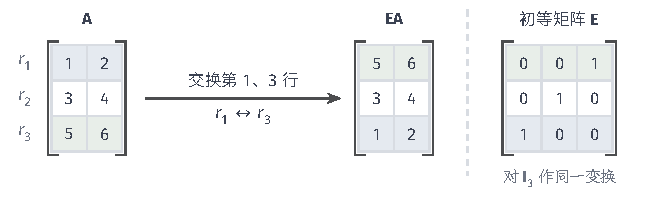
\includegraphics[width=109mm]{figures/02-vectors-matrices-and-multivariate-calculus/01-vectors-and-linear-spaces/tikz/ls-elementary-row-operations/row-swap.pdf}
  \caption{交换两行。左为$\bm A$，中间为交换第$1$、$3$行后的$\bm E\bm A$，右为对$\bm I_3$作同一交换得到的初等矩阵$\bm E$；同色表示同一行内容，换位后颜色随行移动。}
  \label{fig:ls-row-swap}
\end{figure}

第二种是将一行乘以非零数$c$，记作$r_i\leftarrow cr_i$。它把这一行的每个元素放大$c$倍，其余行不动。图~\ref{fig:ls-row-scale}把第$2$行乘以$2$，对应的初等矩阵是对角矩阵$\operatorname{diag}(1,2,1)$。要撤销它，只需把同一行乘以$1/c$。这里必须要求$c\neq0$：乘以$0$会把整行抹成零，原来的数据无法恢复。
\begin{figure}[!htb]
  \centering
  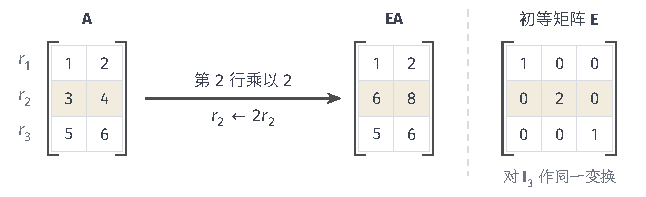
\includegraphics[width=109mm]{figures/02-vectors-matrices-and-multivariate-calculus/01-vectors-and-linear-spaces/tikz/ls-elementary-row-operations/row-scale.pdf}
  \caption{一行乘以非零数。第$2$行（黄色）乘以$2$，其余两行不变；初等矩阵$\bm E=\operatorname{diag}(1,2,1)$只在第$2$个对角元上与$\bm I_3$不同。}
  \label{fig:ls-row-scale}
\end{figure}

第三种是将一行加上另一行的倍数，记作$r_i\leftarrow r_i+cr_k$（$i\neq k$）。被加的一行改变，提供倍数的一行保持不动。图~\ref{fig:ls-row-replace}把第$3$行加上第$1$行的$-5$倍，第$3$行的首个元素$5$变成$0$；后面消元时正是用这种变换把指定位置化为零。对应的初等矩阵是在$\bm I_3$的$(3,1)$位置放上$-5$。撤销时，把第$3$行再加上第$1$行的$5$倍：第$1$行没有变，所以原来加上的量可以原样减回。
\begin{figure}[!htb]
  \centering
  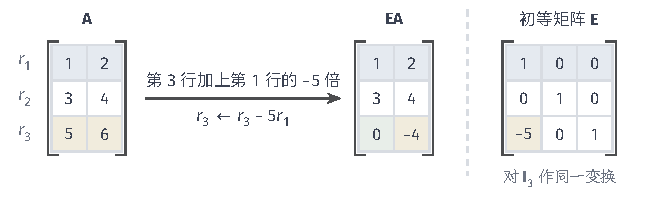
\includegraphics[width=109mm]{figures/02-vectors-matrices-and-multivariate-calculus/01-vectors-and-linear-spaces/tikz/ls-elementary-row-operations/row-replace.pdf}
  \caption{一行加上另一行的倍数。第$3$行（黄色）加上第$1$行（蓝色）的$-5$倍，第$1$行不变，第$3$行首个元素化为$0$（绿色）；初等矩阵$\bm E$只在$(3,1)$位置与$\bm I_3$不同。}
  \label{fig:ls-row-replace}
\end{figure}

三种变换的逆操作仍是同类的初等行变换，对应的初等矩阵就是$\bm E$的逆，所以每个初等矩阵都可逆。接连执行若干次行变换，相当于依次左乘这些初等矩阵，总的效果是左乘它们的乘积，它仍是可逆矩阵。

用初等行变换把矩阵化为阶梯形、求解线性方程组和求逆矩阵的具体做法，放在第~\ref{sec:ls-gaussian-elimination}节与求解方法一起讨论。

\subsection{逆矩阵}
\label{sec:prelim-inverse-matrices}

逆矩阵用来撤销一次矩阵乘法。对$n$阶方阵$\bm A$，若存在$n$阶方阵$\bm B$满足
\[
 \bm A\bm B=\bm B\bm A=\bm I_n,
\]
就称$\bm A$可逆，称$\bm B$为$\bm A$的\term{逆矩阵}（inverse matrix），记作$\bm A^{-1}$。

可逆矩阵给出的方程有唯一解。设$\bm A$可逆。若$\bm A\bm x=\bm y$，两边左乘$\bm A^{-1}$得$\bm x=\bm A^{-1}\bm y$，所以方程至多有一个解；反过来，$\bm x=\bm A^{-1}\bm y$满足$\bm A\bm x=\bm A\bm A^{-1}\bm y=\bm y$。所以方程$\bm A\bm x=\bm y$有唯一解$\bm x=\bm A^{-1}\bm y$。

逆矩阵若存在则唯一。若$\bm B,\bm C$都满足条件，由结合律，
\[
 \bm B=\bm B(\bm A\bm C)=(\bm B\bm A)\bm C=\bm C.
\]
因此记号$\bm A^{-1}$没有歧义。

怎样求逆取决于矩阵的结构。下面先给出对角矩阵和二阶方阵的逆，再说明一般方阵的求逆怎样归结为解方程。

\paragraph{对角矩阵的逆}
每个$d_i\neq0$时，逐个取倒数：
\[
 \operatorname{diag}(d_1,\ldots,d_n)^{-1}=\operatorname{diag}(1/d_1,\ldots,1/d_n).
\]
两个对角矩阵相乘时对角元逐个相乘，所以两侧乘积都是$\bm I_n$。例如$\operatorname{diag}(2,1)^{-1}=\operatorname{diag}(1/2,1)$。若某个$d_i=0$，则$\bm D=\operatorname{diag}(d_1,\ldots,d_n)$左乘任何$\bm B$，都把$\bm B$的第$i$行乘以$0$。于是$\bm D\bm B$的第$i$行是零，不可能等于$\bm I_n$的第$i$行，这时$\bm D$不可逆。

\paragraph{二阶方阵的逆}
$ad-bc\neq0$时，
\[
 \begin{pmatrix}a&b\\c&d\end{pmatrix}^{-1}=\frac1{ad-bc}\begin{pmatrix}d&-b\\-c&a\end{pmatrix}.
\]
直接相乘即可验证两侧乘积都是$\bm I_2$：例如左上元素为$(ad-bc)/(ad-bc)=1$，右上元素为$(-ab+ba)/(ad-bc)=0$。分母$ad-bc$就是下一节的二阶行列式。

\paragraph{一般方阵的逆}
一般方阵没有这样简短的公式。按列看等式$\bm A\bm A^{-1}=\bm I_n$，$\bm A^{-1}$的第$j$列$\bm A^{-1}\bm e_j$正是方程$\bm A\bm x=\bm e_j$的解，所以求逆就是解$n$个系数矩阵相同的线性方程组。怎样用初等行变换一并解这些方程，以及化简失败为什么说明矩阵不可逆，在第~\ref{sec:ls-gaussian-elimination}节讨论；方阵何时可逆，在第~\ref{chap:linear-solution-selection}章系统处理。只求一个方程的解时，通常直接消元或用分解求解，不必先求出整个逆矩阵。

\paragraph{单侧逆}
矩形矩阵没有双侧的逆，但可能从一侧抵消。对$\bm A\in\mathbb R^{m\times d}$，满足$\bm L\bm A=\bm I_d$的$\bm L\in\mathbb R^{d\times m}$称为左逆，满足$\bm A\bm R=\bm I_m$的$\bm R\in\mathbb R^{d\times m}$称为右逆。

两种单侧逆对方程$\bm A\bm x=\bm y$的作用不同。有左逆时，若方程有解，两边左乘$\bm L$得$\bm x=\bm L\bm y$，所以解只能是$\bm L\bm y$。有右逆时，$\bm A(\bm R\bm y)=\bm I_m\bm y=\bm y$，所以$\bm x=\bm R\bm y$总是一个解。

与方阵的逆不同，单侧逆一般不唯一。
\begin{example}[反例：左逆不唯一]
\label{ex:ls-left-inverse-not-unique}
取$\bm A=(1,0)^\top\in\mathbb R^{2\times1}$。对任意实数$c$，令$\bm L=(1,c)\in\mathbb R^{1\times2}$，则
\[
 \bm L\bm A=1\cdot1+c\cdot0=1=\bm I_1.
\]
$\bm A$的第二个坐标是零，$\bm L$的第二个元素无论取什么都不影响乘积。于是每个$c$都给出一个左逆，$\bm A$的左逆有无穷多个。
\end{example}

回到方阵。下面几条规则说明，可逆方阵经过乘积、求逆、数乘和转置以后仍然可逆，并给出逆矩阵的表达式。设$\bm A,\bm B$都是$n$阶可逆方阵。

\paragraph{乘积的逆}
两个可逆方阵的乘积仍然可逆，它的逆是两个因子的逆按相反次序相乘。
\begin{theorem}[乘积的逆]
\label{thm:ls-inverse-product}
设$\bm A,\bm B$都是$n$阶可逆方阵，则$\bm A\bm B$可逆，且
\begin{equation}
 (\bm A\bm B)^{-1}=\bm B^{-1}\bm A^{-1}.
 \label{eq:ls-inverse-product}
\end{equation}
\end{theorem}
\begin{proof}
由矩阵乘法的结合律，
\[
 \begin{gathered}
 (\bm A\bm B)(\bm B^{-1}\bm A^{-1})=\bm A(\bm B\bm B^{-1})\bm A^{-1}=\bm A\bm A^{-1}=\bm I_n,\\
 (\bm B^{-1}\bm A^{-1})(\bm A\bm B)=\bm B^{-1}(\bm A^{-1}\bm A)\bm B=\bm B^{-1}\bm B=\bm I_n.
 \end{gathered}
\]
按逆矩阵的定义，$\bm B^{-1}\bm A^{-1}$是$\bm A\bm B$的逆；由逆矩阵的唯一性，式~\eqref{eq:ls-inverse-product}成立。
\end{proof}
次序反转是因为$\bm A\bm B\bm x$先作用$\bm B$、再作用$\bm A$，撤销时要先撤销后作用的$\bm A$，再撤销$\bm B$。

\paragraph{逆的逆}
\[
 (\bm A^{-1})^{-1}=\bm A.
\]
在定义中，$\bm A$与$\bm A^{-1}$的地位对称：$\bm A^{-1}\bm A=\bm A\bm A^{-1}=\bm I_n$同样说明$\bm A$是$\bm A^{-1}$的逆。

\paragraph{数乘的逆}
\[
 (c\bm A)^{-1}=c^{-1}\bm A^{-1}\qquad(c\neq0).
\]
直接相乘：$(c\bm A)(c^{-1}\bm A^{-1})=(cc^{-1})\bm A\bm A^{-1}=\bm I_n$，反方向同理。

\paragraph{转置的逆}
\[
 (\bm A^\top)^{-1}=(\bm A^{-1})^\top.
\]
由乘积的转置，$\bm A^\top(\bm A^{-1})^\top=(\bm A^{-1}\bm A)^\top=\bm I^\top=\bm I$，反方向同理，所以$(\bm A^{-1})^\top$就是$\bm A^\top$的逆。

\subsection{矩阵的幂}
\label{sec:ls-matrix-power-rules}

同一个方阵反复作用，就得到矩阵的幂。对$d$阶方阵$\bm A$，$\bm A^k$定义为$k$个$\bm A$连乘（$k\geq1$），并规定$\bm A^0=\bm I_d$。$\bm A$可逆时，再定义负幂$\bm A^{-k}=(\bm A^{-1})^k$。非方阵不能与自身相乘，所以没有矩阵幂。

矩阵的幂是反复的矩阵乘法，不是逐元素乘方。下面的例子说明两者的差别。
\begin{example}[矩阵的平方不是逐元素平方]
\label{ex:ls-matrix-square-shear}
取
\[
 \bm A=\begin{pmatrix}1&1\\0&1\end{pmatrix},
\]
按矩阵乘法计算它的平方：
\[
 \bm A^2=\begin{pmatrix}1&1\\0&1\end{pmatrix}\begin{pmatrix}1&1\\0&1\end{pmatrix}
 =\begin{pmatrix}1\cdot1+1\cdot0&1\cdot1+1\cdot1\\0\cdot1+1\cdot0&0\cdot1+1\cdot1\end{pmatrix}
 =\begin{pmatrix}1&2\\0&1\end{pmatrix}.
\]
右上角的元素变为$2$，逐元素平方却只会得到$1^2=1$。差别在于$\bm A^2$的右上角是第一行与第二列的内积$1\cdot1+1\cdot1$，同时用到了两个元素。继续相乘，右上角每次增加$1$。
\end{example}

有两类矩阵由幂的关系刻画。满足$\bm A^2=\bm A$的方阵称为\term{幂等}（idempotent）矩阵，它作用一次与作用多次效果相同。存在正整数$s$使$\bm N^s=\bm0$的方阵称为\term{幂零}（nilpotent）矩阵。下面各举一例。
\begin{example}[幂等矩阵与幂零矩阵]
\label{ex:ls-idempotent-nilpotent}
看两个二阶矩阵
\[
\bm P=\operatorname{diag}(1,0),\qquad
\bm N=\begin{pmatrix}0&1\\0&0\end{pmatrix}
\]
对$\bm u\in\mathbb R^2$的作用。$\bm P\bm u=(u_1,0)^\top$只保留第一个坐标；$(u_1,0)^\top$再经过$\bm P$，第一个坐标照样保留，第二个坐标本来就是零，结果不变，所以$\bm P^2=\bm P$。$\bm N\bm u=(u_2,0)^\top$把第二个坐标移到第一个位置，并把第二个位置清零；再作用一次时，$\bm N$丢掉第一个坐标$u_2$，而第二个坐标已是零，得$\bm N(u_2,0)^\top=(0,0)^\top$。直接相乘也得到
\[
 \bm N^2=\begin{pmatrix}0&1\\0&0\end{pmatrix}\begin{pmatrix}0&1\\0&0\end{pmatrix}=\begin{pmatrix}0&0\\0&0\end{pmatrix}.
\]
所以$\bm P$是幂等矩阵；$\bm N$本身不是零矩阵，平方却为零，是幂零矩阵。
\end{example}

\subsubsection{幂的性质}
同一矩阵的幂按结合律满足与实数幂相同的指数法则。设$\bm A$为方阵，$m,n$为非负整数；$\bm A$可逆时，$m,n$可取任意整数。

\paragraph{同底幂相乘}
\[
 \bm A^m\bm A^n=\bm A^{m+n}.
\]
由结合律，两边都是同样个数的$\bm A$（或$\bm A^{-1}$）连乘；指数异号时，相邻的$\bm A\bm A^{-1}$逐对消去。交换$m,n$可见，同一矩阵的不同次幂彼此可以交换。不同矩阵则不一定交换，因此
\[
 (\bm A+\bm B)^2=\bm A^2+\bm A\bm B+\bm B\bm A+\bm B^2,
\]
只有$\bm A\bm B=\bm B\bm A$时，才能把中间两项合成$2\bm A\bm B$。这与标量平方公式的差别来自乘法的次序。

\paragraph{幂的幂}
\[
 (\bm A^m)^n=\bm A^{mn}.
\]
左边是$n$组、每组$m$个因子的连乘，由结合律去掉括号即得。

\paragraph{负幂与逆相容}
\[
 (\bm A^k)^{-1}=(\bm A^{-1})^k=\bm A^{-k}.
\]
对$k$个相同因子反复使用式~\eqref{eq:ls-inverse-product}即得。
